\chapter{Réalisation du Sprint 1 : Authentification et Gestion des Utilisateurs}

\section*{Introduction}
\addcontentsline{toc}{section}{Introduction}

Le premier sprint du projet EduGenius a été consacré à la mise en place du système d'authentification et des mécanismes de sécurité fondamentaux. Ces fonctionnalités constituent la pierre angulaire de la plateforme, visant à garantir la protection des données sensibles et à assurer un contrôle d'accès strict selon les rôles d'administrateur, d'enseignant et d'étudiant. Ce cycle de développement s'est structuré autour de plusieurs User Stories clés, couvrant notamment l'inscription des nouveaux membres, la connexion sécurisée via des protocoles modernes et la gestion de la récupération des comptes. 

Ce chapitre détaille l'ensemble des étapes ayant conduit à la concrétisation de ce premier incrément logiciel. Nous présenterons d'abord le backlog spécifique à ce sprint et l'analyse fonctionnelle des besoins identifiés. Ensuite, nous aborderons la conception technique et la réalisation des interfaces utilisateurs développées sous Next.js. Enfin, ce chapitre se conclura par une présentation des tests unitaires et d'intégration permettant de valider la robustesse et la fiabilité des fonctionnalités implémentées avant leur déploiement.


\section{Backlog du Sprint 1}

Le backlog du Sprint 1 présente les six User Stories (US) prioritaires liées à l'authentification, à la gestion des utilisateurs et aux fondations techniques (tableau de bord unifié et responsive). Ces US ont été sélectionnées pour leur impact métier et leur caractère transverse, structurant ainsi les développements clés de ce premier incrément.

Le tableau \ref{tab:sprint1_backlog} détaille chaque US avec ses critères d'acceptation et sa priorité. Les US-01 (Connexion sécurisée), US-02 (Gestion des rôles), US-04 (Création des classes), US-39 (Dashboard unifié) et US-41 (Interface responsive) sont classées comme « Haute » priorité en raison de leur rôle central dans la plateforme. L'US-03 (Profil utilisateur) est priorisée « Moyenne », car dépendante des précédentes mais non bloquante pour le reste du sprint. Les tâches techniques sous‑jacentes (chiffrement des mots de passe, génération de token JWT, adaptation CSS responsive) répondent aux exigences de sécurité et d'expérience utilisateur.

\begin{table}[H]
\centering
\small
\begin{tabularx}{\textwidth}{|c|l|X|c|}
\hline
\textbf{ID} & \textbf{Titre} & \textbf{Critères d’acceptation} & \textbf{Priorité} \\
\hline
US-01 & Connexion sécurisée & L'utilisateur peut se connecter avec les identifiants fournis par l'administrateur ; un token JWT valide est délivré. & Haute \\
\hline
US-02 & Gestion des rôles & L'administrateur peut attribuer les rôles (Admin, Enseignant, Étudiant) lors de la création ou modification d'un compte. & Haute \\
\hline
US-03 & Profil utilisateur & L'utilisateur peut consulter et modifier ses informations (nom, photo, mot de passe). & Moyenne \\
\hline
US-04 & Création et gestion des classes & L'administrateur peut créer, modifier ou supprimer une classe et y assigner des étudiants et un enseignant. & Haute \\
\hline
US-39 & Dashboard unifié & L'utilisateur dispose d'un tableau de bord personnalisé affichant son planning, les deadlines et les sessions à venir. & Haute \\
\hline
US-41 & Interface responsive & La plateforme est utilisable sur mobile, tablette et desktop sans perte de fonctionnalité. & Haute \\
\hline
\end{tabularx}
\caption{User Stories du Sprint 1 (Authentification et Sécurité)}
\label{tab:sprint1_backlog}
\end{table}

\section{Analyse}

\subsection{Diagramme de cas d’utilisation du Sprint 1}
Le diagramme de cas d’utilisation présenté en figure \ref{fig:usecase_sprint1} illustre les interactions entre l’utilisateur (non authentifié ou authentifié) et le système pour les fonctionnalités d’authentification et de gestion de profil.

\begin{figure}[H]
    \centering
    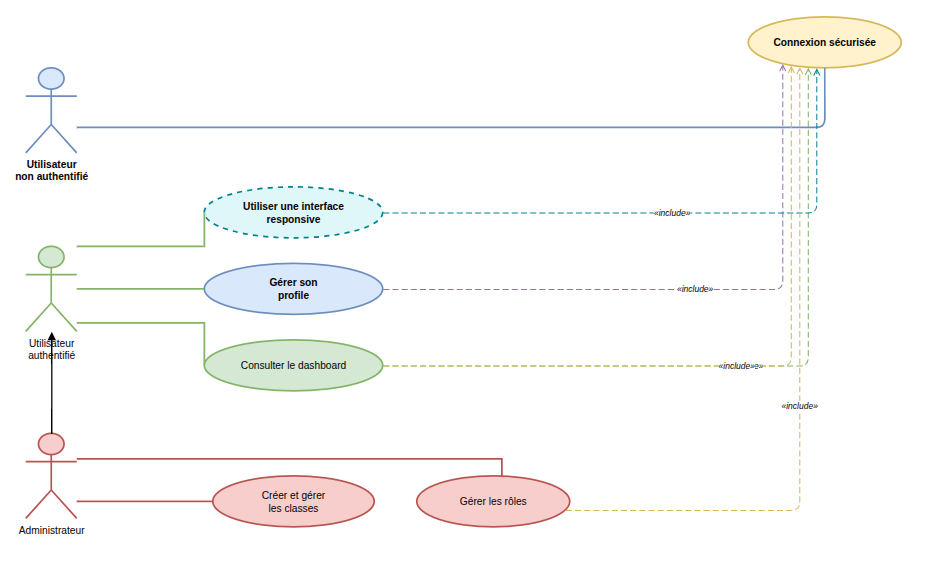
\includegraphics[width=1\textwidth]{images/sprint_1_usecase_diagram.png}
    \caption{Diagramme de cas d’utilisation – Authentification et sécurité}
    \label{fig:usecase_sprint1}
\end{figure}

\subsection{Description textuelle des cas d’utilisation}

Cette section décrit de manière structurée les scénarios nominaux et alternatifs pour chaque cas d'utilisation du sprint. Chaque cas (par exemple « S’authentifier ») est décomposé en éléments clés : acteur, préconditions, postconditions et étapes du scénario nominal. Le scénario nominal de connexion inclut la génération d’un token JWT, tandis qu’un échec (scénario alternatif) déclenche un message d’erreur générique. Les postconditions garantissent des états système cohérents, comme l’accès au tableau de bord après authentification.

\subsubsection{Le cas d’utilisation « S’authentifier »}
\begin{itemize}
    \item \textbf{Acteur} : Utilisateur non authentifié (futur élève, enseignant ou administrateur).
    \item \textbf{Préconditions} : Les comptes enseignants et étudiants ont été créés au préalable par l’administrateur ; le compte administrateur existe en base de données. L’utilisateur a reçu ses identifiants.
    \item \textbf{Postconditions} : Un token JWT valide est généré et l’utilisateur accède à son tableau de bord personnalisé.
    \item \textbf{Scénario nominal} :
    \begin{enumerate}
        \item L’utilisateur saisit son email et son mot de passe sur la page de connexion.
        \item Le système recherche l’utilisateur par email dans la collection MongoDB.
        \item Le système compare le mot de passe fourni avec le hachage bcrypt stocké.
        \item Le système génère un token JWT contenant l’identifiant, le rôle et la date d’expiration.
        \item Le token est retourné au client (cookie sécurisé / localStorage).
        \item L’utilisateur est redirigé vers son tableau de bord (adapté à son rôle).
    \end{enumerate}
    \item \textbf{Alternatives / Erreurs} :
    \begin{itemize}
        \item \textbf{Email inconnu ou mot de passe incorrect} : message générique « Identifiants invalides ».
        \item \textbf{Compte désactivé} : message invitant à contacter l’administrateur.
        \item \textbf{Token expiré} : l’utilisateur est invité à se reconnecter.
    \end{itemize}
\end{itemize}

\subsubsection{Le cas d’utilisation « Gérer son profil »}
\begin{itemize}
    \item \textbf{Acteur} : Utilisateur authentifié (élève, enseignant ou administrateur).
    \item \textbf{Préconditions} : L’utilisateur est connecté.
    \item \textbf{Postconditions} : Les informations modifiables (nom, photo, mot de passe) sont mises à jour en base.
    \item \textbf{Scénario nominal} :
    \begin{enumerate}
        \item L’utilisateur accède à la page « Mon profil ».
        \item Le système affiche les données actuelles.
        \item L’utilisateur modifie les champs autorisés et valide.
        \item Le système vérifie la validité des nouvelles données (unicité de l’email, complexité du mot de passe).
        \item Le système enregistre les modifications et affiche un message de confirmation.
    \end{enumerate}
    \item \textbf{Alternatives / Erreurs} :
    \begin{itemize}
        \item \textbf{Nouvel email déjà utilisé} : erreur et refus de la modification.
        \item \textbf{Mot de passe trop faible} : réaffichage des règles de sécurité.
    \end{itemize}
\end{itemize}

\subsubsection{Le cas d’utilisation « Consulter le tableau de bord »}
\begin{itemize}
    \item \textbf{Acteur} : Utilisateur authentifié.
    \item \textbf{Préconditions} : L’utilisateur est connecté.
    \item \textbf{Postconditions} : Le tableau de bord personnalisé est affiché (planning, notifications, évaluations à venir).
    \item \textbf{Scénario nominal} :
    \begin{enumerate}
        \item Après connexion ou en cliquant sur « Tableau de bord », le système agrège les données pertinentes.
        \item Pour un étudiant : affichage des cours à venir, devoirs, présences.
        \item Pour un enseignant : listes de ses classes, appels vidéo planifiés, quiz à corriger.
        \item Pour l’administrateur : statistiques générales, gestion des comptes.
    \end{enumerate}
    \item \textbf{Alternatives / Erreurs} :
    \begin{itemize}
        \item \textbf{Données non disponibles} : affichage de messages informatifs (ex. « Aucun cours planifié »).
    \end{itemize}
\end{itemize}

\subsubsection{Le cas d’utilisation « Utiliser l’interface responsive »}
\begin{itemize}
    \item \textbf{Acteur} : Tout utilisateur (non ou authentifié).
    \item \textbf{Préconditions} : L’utilisateur accède à la plateforme depuis un mobile, une tablette ou un ordinateur.
    \item \textbf{Postconditions} : La mise en page s’adapte automatiquement à la taille de l’écran sans perte de fonctionnalité.
    \item \textbf{Scénario nominal} :
    \begin{enumerate}
        \item L’utilisateur ouvre l’application sur un smartphone.
        \item Les styles CSS réorganisent les éléments (menu en accordéon, polices lisibles).
        \item Toutes les actions (connexion, consultation de cours, quiz) restent accessibles.
    \end{enumerate}
    \item \textbf{Alternatives / Erreurs} :
    \begin{itemize}
        \item \textbf{Navigation dégradée} : si une fonctionnalité n’est pas adaptée, un message invite à passer sur un écran plus large.
    \end{itemize}
\end{itemize}

\subsubsection{Le cas d’utilisation « Gérer les utilisateurs » (administrateur)}
\begin{itemize}
    \item \textbf{Acteur} : Administrateur.
    \item \textbf{Préconditions} : L’administrateur est connecté.
    \item \textbf{Postconditions} : Un compte enseignant ou étudiant est créé (ou modifié/supprimé) dans la collection \texttt{User}.
    \item \textbf{Scénario nominal (création)} :
    \begin{enumerate}
        \item L’administrateur accède à l’interface « Gestion des utilisateurs ».
        \item Il clique sur « Ajouter un utilisateur » et remplit le formulaire (nom, prénom, email, rôle enseignant/étudiant).
        \item Le système vérifie l’unicité de l’email et la validité des champs.
        \item Le système génère un mot de passe temporaire sécurisé, le hache et enregistre l’utilisateur.
        \item Un email contenant les identifiants (email + mot de passe temporaire) est envoyé à l’utilisateur.
        \item L’utilisateur devra changer son mot de passe lors de la première connexion.
    \end{enumerate}
    \item \textbf{Alternatives / Erreurs} :
    \begin{itemize}
        \item \textbf{Email déjà existant} : refus de création, message d’erreur.
        \item \textbf{Rôle invalide} : l’administrateur ne peut pas créer un autre administrateur via cette interface (réservé à une procédure manuelle).
    \end{itemize}
\end{itemize}

\subsubsection{Le cas d’utilisation « Créer et gérer les classes » (administrateur)}
\begin{itemize}
    \item \textbf{Acteur} : Administrateur.
    \item \textbf{Préconditions} : L’administrateur est connecté. Les départements, programmes et années académiques existent.
    \item \textbf{Postconditions} : Une classe est créée, modifiée ou supprimée, avec assignation d’un enseignant et d’étudiants.
    \item \textbf{Scénario nominal} :
    \begin{enumerate}
        \item L’administrateur remplit le formulaire de création (nom, code, département, programme, année).
        \item Il sélectionne les étudiants inscrits et l’enseignant responsable.
        \item Le système ajoute la classe dans MongoDB et met à jour les références.
    \end{enumerate}
    \item \textbf{Alternatives / Erreurs} :
    \begin{itemize}
        \item \textbf{Code de classe déjà existant} : message d’erreur demandant un autre code.
        \item \textbf{Suppression d’une classe contenant des cours actifs} : confirmation requise.
    \end{itemize}
\end{itemize}
\begin{itemize}
    \item \textbf{Acteur} : Utilisateur authentifié (étudiant, enseignant ou admin).
    \item \textbf{Préconditions} : L’utilisateur est connecté.
    \item \textbf{Postconditions} : Les informations du profil sont mises à jour selon les modifications demandées.
    \item \textbf{Scénario nominal (consultation)} :
    \begin{enumerate}
        \item L’utilisateur accède à son espace « Mon profil ».
        \item Le système affiche les informations actuelles (nom, prénom, email, photo, etc.).
    \end{enumerate}
    \item \textbf{Scénario nominal (modification)} :
    \begin{enumerate}
        \item L’utilisateur modifie un ou plusieurs champs modifiables (nom, photo, mot de passe).
        \item Le système valide les nouvelles données (format, unicité de l’email si modifié).
        \item Le système enregistre les changements.
        \item Un message de confirmation est affiché.
    \end{enumerate}
    \item \textbf{Alternatives / Erreurs} :
    \begin{itemize}
        \item \textbf{Nouvel email déjà utilisé} : erreur et refus de la modification.
        \item \textbf{Nouveau mot de passe trop faible} : le système exige des critères de robustesse.
    \end{itemize}
\end{itemize}

\section{Conception}
\subsection{Diagramme de séquence du cas « S’authentifier »}
\begin{figure}[H]
    \centering
    % \includegraphics[width=0.8\textwidth]{images/sequence_auth.png}
    \caption{Diagramme de séquence de l’authentification JWT}
    \label{fig:sequence_auth}
\end{figure}

\subsection{Diagramme de séquence du cas « Consulter profil »}
\begin{figure}[H]
    \centering
    % \includegraphics[width=0.8\textwidth]{images/sequence_profil.png}
    \caption{Diagramme de séquence de la consultation du profil}
    \label{fig:sequence_profil}
\end{figure}

\subsection{Diagramme de classes du Sprint 1}
\begin{figure}[H]
    \centering
    % \includegraphics[width=\textwidth]{images/class_sprint1.png}
    \caption{Diagramme de classes – Modèle utilisateur et authentification}
    \label{fig:class_sprint1}
\end{figure}

\subsection{Représentation graphique de la base de données}
\begin{figure}[H]
    \centering
    % \includegraphics[width=\textwidth]{images/mongodb_sprint1.png}
    \caption{Schéma des collections MongoDB pour le sprint 1}
    \label{fig:mongodb_sprint1}
\end{figure}

\section{Réalisation}
\subsection{Interface d’inscription}
\begin{figure}[H]
    \centering
    % \includegraphics[width=0.7\textwidth]{images/register_ui.png}
    \caption{Formulaire d’inscription}
    \label{fig:register_ui}
\end{figure}

\subsection{Interface de connexion}
\begin{figure}[H]
    \centering
    % \includegraphics[width=0.7\textwidth]{images/login_ui.png}
    \caption{Page de connexion}
    \label{fig:login_ui}
\end{figure}

\subsection{Interface de réinitialisation de mot de passe}
\begin{figure}[H]
    \centering
    % \includegraphics[width=0.7\textwidth]{images/reset_ui.png}
    \caption{Formulaire de réinitialisation}
    \label{fig:reset_ui}
\end{figure}

\subsection{Interface profil utilisateur}
\begin{figure}[H]
    \centering
    % 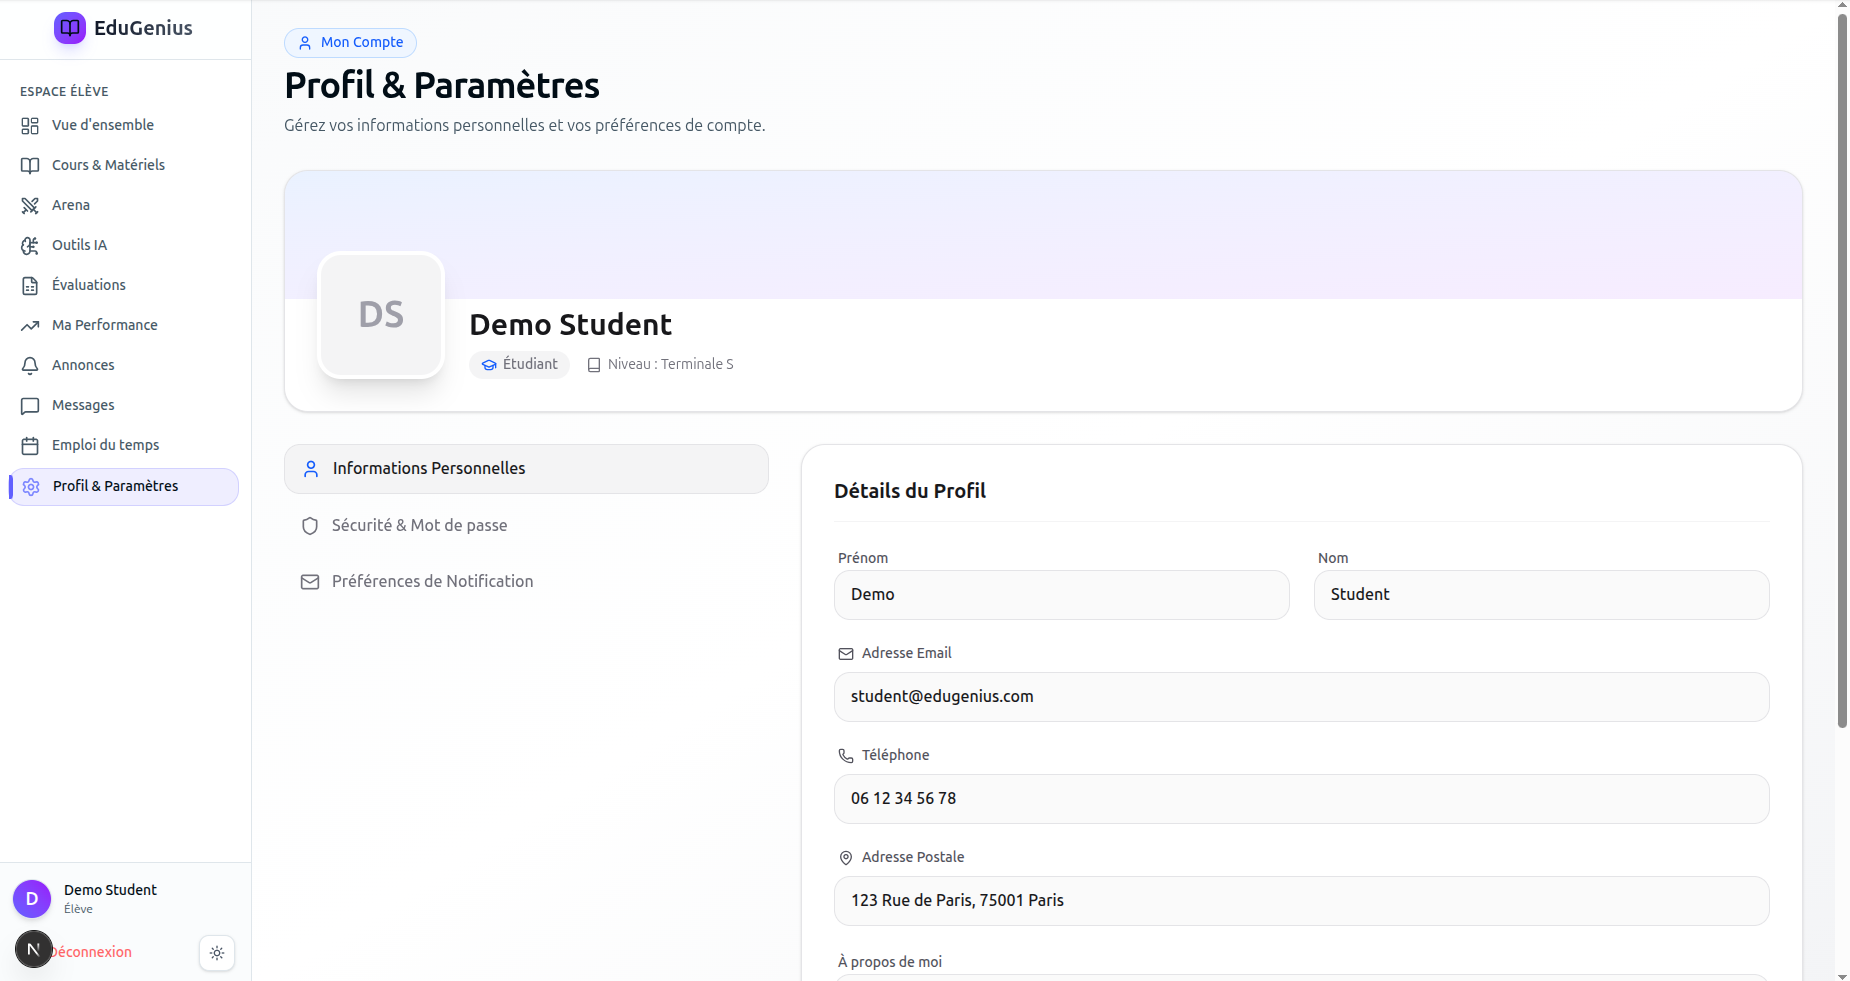
\includegraphics[width=0.7\textwidth]{images/profile_ui.png}
    \caption{Page de profil}
    \label{fig:profile_ui}
\end{figure}

\section{Tests}
\subsection{Tests unitaires}
\ldots

\subsection{Tests d’intégration}
\ldots

\subsection{Tests fonctionnels}
\ldots

\section{Conclusion}
\ldots